\documentclass[11pt]{article}
\usepackage{graphicx}  % this is the up-to-date package for all figures
\usepackage{float}	% allows use of 'H' command
\usepackage{hyperref}	% needed to add hyperlinks
\hypersetup{
  colorlinks=true,
  linkcolor=blue,
  filecolor=magenta,
  urlcolor=cyan,
}

% these are some custom control of the page size and margins
% \topmargin= 0.2in  % these 1st two may be needed for some computers
%\textheight=8.75in
\textwidth=6.5in
\oddsidemargin=0cm
\evensidemargin=0cm

% this is where the actual document itself (rather than control statements) begins:

\begin{document}

\pagestyle{myheadings}


\title{Apollo:\\
Shoot the Moon}


\author{Corey Mutnik \\
{\it Computational Physics 305, University of Hawaii at Manoa} }


\date{April 14, 2015}

\maketitle   




\abstract{ The objective of this mission was to have a spacecraft leave Earths parking orbit (175 km), venture to the Moon, 
and return back to Earth.  To do this a program with proper force laws needed to be written.  It was necessary that the 
program also began with specific inital parameters.

}

\section{Introduction}
Here we began by modeling the Earth-Moon system using the gravitational forces of one body on the other.  Inorder to properly 
model the system we had to solve for the center of mass (barycenter).  The barycenter is the point that each object in our system 
orbits.  Using Newton's Force Laws we modeled the force each object had on the other:
\begin{equation}
\label{fME}
\vec {F}_{1,2} ~=~ -\vec {F}_{2,1} ~=~ \frac{GM_{1}M_{2}}{| \vec {r_1} - \vec {r_2} |^3}(\vec {r_1} - \vec {r_2}) 
\end{equation}
where $\vec {F}_{1,2}$ is the force of one body acting on the other, G is the Gravitational constant, 
$M_{1}$ is mass of object one, 
$M_{2}$ is the mass of object two, $\vec {r_1}$ and $\vec {r_2}$ are the respective position vectors of each body.  
From these standard force laws the acceleration each body caused on the other was able to be determined.  This was necessary 
in order to impliment the Runge-Kutta method of numerical analysis.




To force structre on the system, Earth was placed at the proper distance below the barycenter.  The Moon's inital location was  
located in the plane, above the barycenter.
\begin{equation}
\label{rEb}
r_{E} = \frac {M_m}{M_{m}+M_{E}}D
\end{equation}

\begin{equation}
\label{rMb}
r_{m} = \frac {M_E}{M_{m}+M_{E}}D
\end{equation}
where $r_{E}$ is the distance from the center of the Earth to the barycenter, $r_{m}$ is the distance from the center of the 
Moon to the barycenter, $M_{m}$ is the mass of the moon, $M_{E}$ is the mass of the Earth, and D is the Earth-Moon distance.  
Knowing $M_{E} >> M_{m}$ tells us that the barycenter is located very close to the center of mass of the Earth.  Once a proper 
Earth-Moon system was modeled we introduced a third body, the Apollo 13 spacecraft.  The objective was to simulate the actual 
flight path of the Apollo 13 mission.
\begin{figure}[H]
  \begin{center}
\centerline{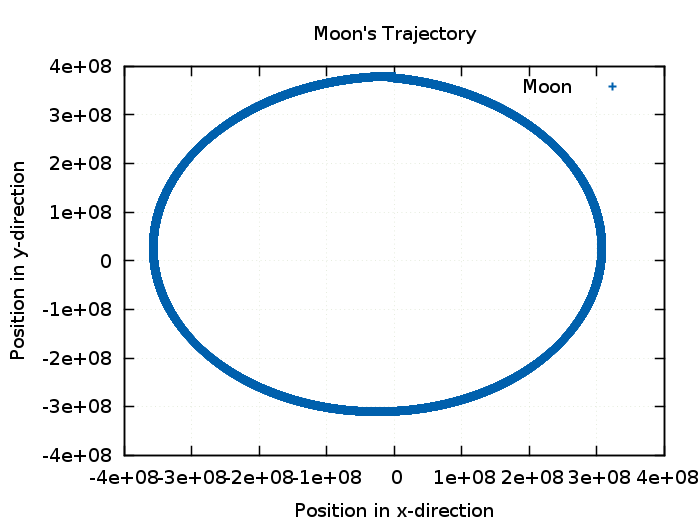
\includegraphics[width=3.5in]{1moonorbit.png}}
\caption{\it \small{The orbit of the moon, about the barycenter of the Earth-Moon system \label{fig1}}}
  \end{center}
\end{figure}
  Figure 1 is a graphical representation of the path traced out by the Moon's orbit,
about the barycenter, in one sidereal Earth-Moon orbital period of 27.322 days.


\section{Computational problem}
During the Apollo 13 mission an issue with the No. 2 oxygen tank force the mission to be modified.  Instead of landing on the 
moon the astronauts aboard were forced to make a course a correction.  It was this correction that led to their gravitational 
slingshot around the Moon.  After tracing out a figure-eight flight pattern the crew was able to land back on Earth safely.

\begin{figure}[H]
  \begin{center}
\centerline{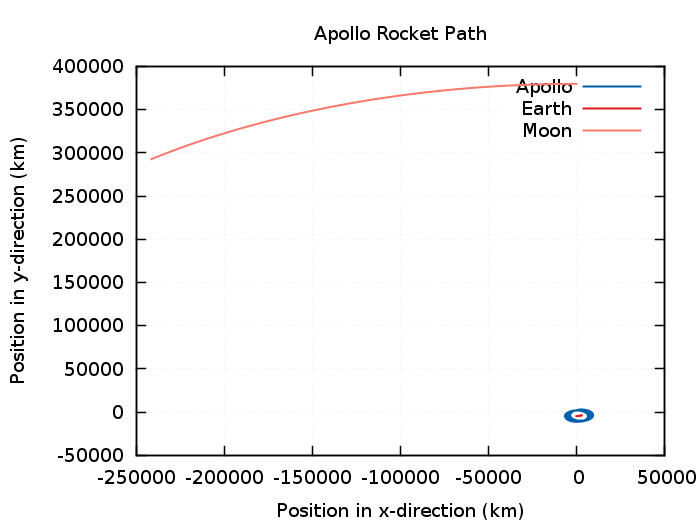
\includegraphics[width=3.5in]{3days.png}}
\caption{\it \small{The Earth-Moon system with a satellite orbiting the Earth \label{fig2}}}
  \end{center}
\end{figure}
Figure 2 shows the orbits of the Earth, Moon, and Apollo spacecraft in parking orbit above the Earth over a period of 3 days.  
In order to model the path of Apollo, as it ventured out of Earths parking orbit, a change in velocity was necessary.  After 
summing the velocity of the spacecraft with that of Earths, a correction had to be made.  For simplicity, the newly added 
velocity was considered to be instantaneous.  By adding more velocity Apollo broke free of Earths parking orbit and began
its transit to the moon.  


The challenge was in uncovering the correct magnitude and direction of the necessary velocity 
correction.  When done properly the spacecraft would loop around the Moon and return the onboard astronauts safely to Earth.  
Computationally, this is no easy task.  First an attempt at a Hohmann Transfer Orbit was made.  In such a simplistic 
scenario this approach quickly proved to surpass our programming capabilities.  In order to achieve the desired goal a 
trial and error method was implemented.  Our first task was to hit the moon.



\section{Results}

\begin{figure}[H]
 \centerline{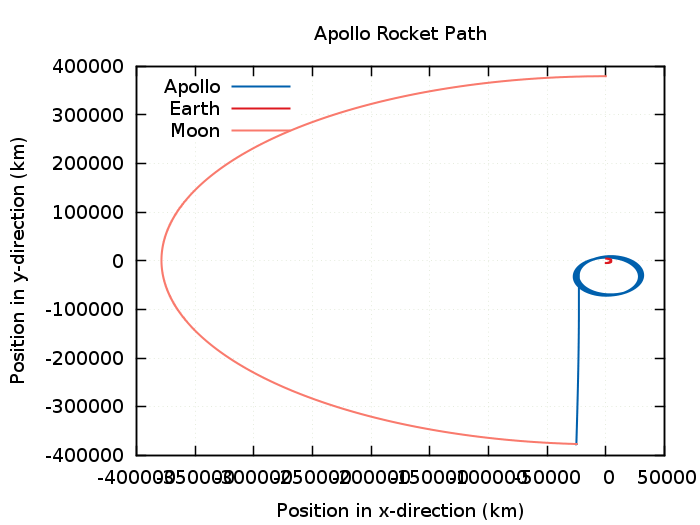
\includegraphics[width=3.0in]{mooncrash.png}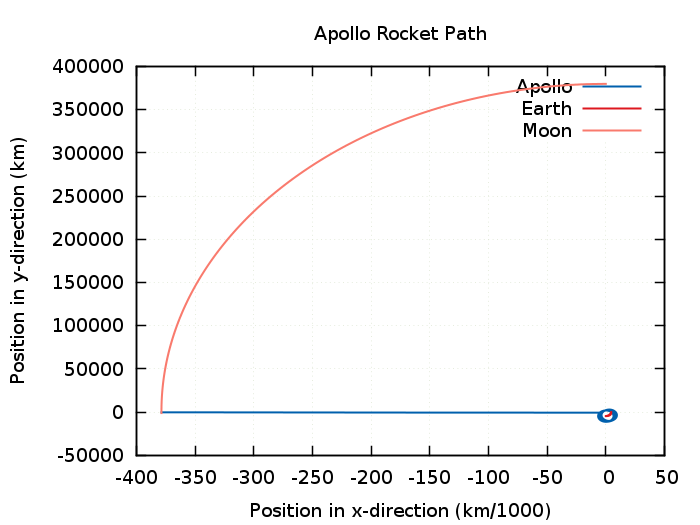
\includegraphics[width=3.0in]{shotleft.png}}
\caption{\it \small{Two different trajectories that cause a lunar crash \label{fig3}}}
\end{figure}

\begin{figure}[H]
  \begin{center}
\centerline{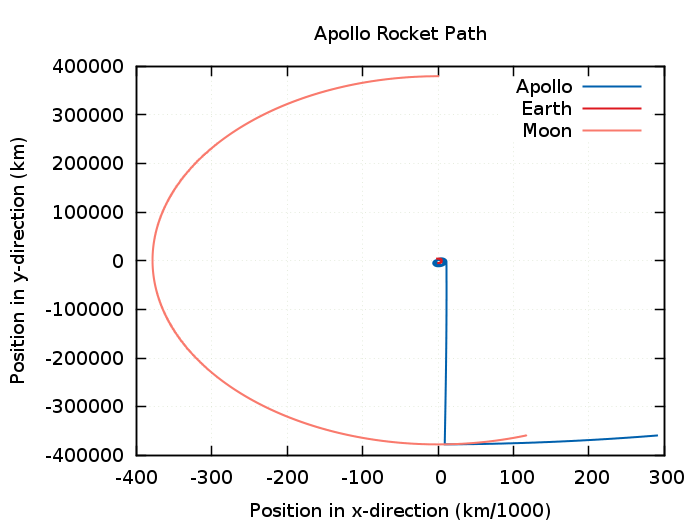
\includegraphics[width=3.5in]{fail.png}}
\caption{\it \small{The Apollo 13 spacecraft unable to orbit the moon \label{fig4}}}
  \end{center}
\end{figure}


\section{Analysis}
Figure 3 depicts the Apollo spacecraft leaving Earths parking orbit and crashing into the Moon, using two different 
changes in velocity.  In order to do this the 
orbital mechanics of each body in the system had to be taken into account.  Once the arrival time was calculated it was 
possible to have the spacecraft orbit the Moon.  This called for another instantaneous change in the velocity.  Once a possible 
lunar orbital velocity is determined the task of brining Apollo 13 back to Earth is done with another instantaneous velocity 
change.  If done correctly, this simulation will end with the safe return of all the onboard astronauts intact.


As seen in figure 4, it is no simple task to catch the orbit of the moon.  Even after crashing into the moons surface it proved 
to difficult to have the spacecraft orbit the moon.  Without the ability to wrap around the moon my program was not capable 
of returning the Apollo 13 rocket and its crew back to Earth.



\section{Conclusion}

Even after simplifications were made the instantaneous velocity corrections were not easy to determine.  More often than not,
the spacecraft would miss the Moon entirely.  In some simulations the velocity correction was to small.  This would have lead 
to the death of all the astronauts due to starvation and dehydration, as they drifted between Earth and the Moon.  This 
simulation began with Apollo already in orbit.  Having a rocket reach the Moon is no easy task.  To get men from Earth to the 
Moon and safely back again is a task few have ever achieved.


% the following \setlength is to force the bibliography to have no
% paragraph indentations.Can use vairous units--cm are used here.
\setlength{\parindent}{0cm}

\begin{thebibliography}{99}  % the trailing 99 controls some obscure format--just use

\bibitem{Landau} R. H. Landau and M. J. Paez, "Computational Physics, Problem Solving with Computers," (Wiley: New York) 1997.


\bibitem{Gorham} Gorham, Peter. "Physics 305 Differential Equations." P305lab7. Phys.hawaii.edu, 7 Apr. 2015. Web. 8 Apr. 2015.

\bibitem{Apollo}  "John F. Kennedy Space Center - Apollo 13." John F. Kennedy Space Center - Apollo 13. N.p., 4 June 2002. Web. 10 Apr. 2015.

\end{thebibliography}

\section*{Acknowledgements}
All programs developed in modeling the motion of this projectile were written with the aid of Landau [1] and Gorham [2].



\end{document}

